Основой современного ассистента является большая языкова модель. Термин большая на текущий момент
означает число параметров модель большее одного миллиарда. Таким образом, физическая запись модель требует
значительно ресурса памяти большое нескольких гигабайт, что и послужило причиной названия.  

Обучение языковых моделей для задач ассистирования разделяется на два этапа предобучение (\textit{англ.} pretrain) и инструкционное дообучение.
В ходе первого этапа модель обучается синтаксической структуре языка. 
Во втором обучается под руководством эксперта на специализированных корпусах инструкций. Таковыми, например, могут являться
дача структурированных определений, изложение информации в специальной стилистической форме, поиск ключевых слов в массивном тексте.

\begin{figure}[h]
    \centering
    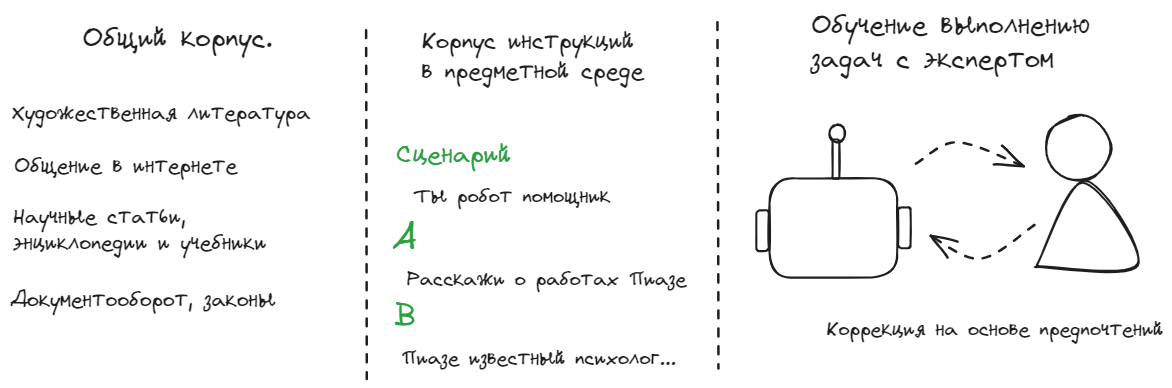
\includegraphics[width=0.5\textwidth]{assets/work/arch/learning.excalidraw.png}
    \caption{Обучение разбито на три ключевых этапа: подготовка, адаптация на корпусе}
    \label{train}
\end{figure}


Предобучение требует значительных вычислительных ресурсов, 
не всегда доступных в образовательных и научных
целях. В связи с этим компании, обладающие достаточным
ресурсом выкладывают свои модели в общий доступ \cite{jiang2023mistral}\cite{jiang2024mixtral}\cite{touvron2023llama}


Для оценки способностей языковых моделей создаются специальные системы тестирования количественно \begin{itemize}
    \item способности к пересказу
    \item умение переводить
    \item  понимание животного и растительного мера 
    \item решение аналитических задач 
\end{itemize}


\begin{figure}[h]
    \centering
    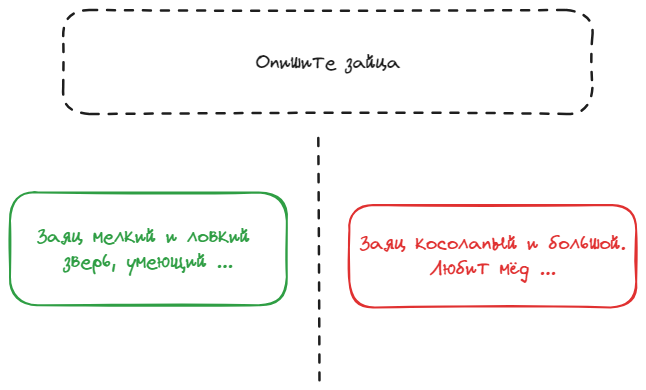
\includegraphics[width=0.5\textwidth]{assets/work/arch/instruction.excalidraw.png}
    \caption{Адаптация выполнять задачи проходит через взаимодействие с пользователем и работу эксперта}
    \label{instruction}
\end{figure}

Для сравнения моделей также используется техника попарного сравнения модели. 
Таким образом, исходя из предпочтений пользователей, выносится оценка по системе Эло.

В ходе исследования было выявлено, что современный ассистент без дополнительного обучения на специализированном 
корпусе не справляется с долгосрочным планированием образовательной траектории.

Для адаптации открытой реализации для работы с детьми необходимо создание формата и предмета коммуникации.

Бранные слова были исключены с помощью библиотеки PyMorphy \cite{Korobov2015morph}, выделяющую нормальную форму слова для сравнения
с опорным корпусом неэтичных слов.

\begin{figure}[h]
    \centering
    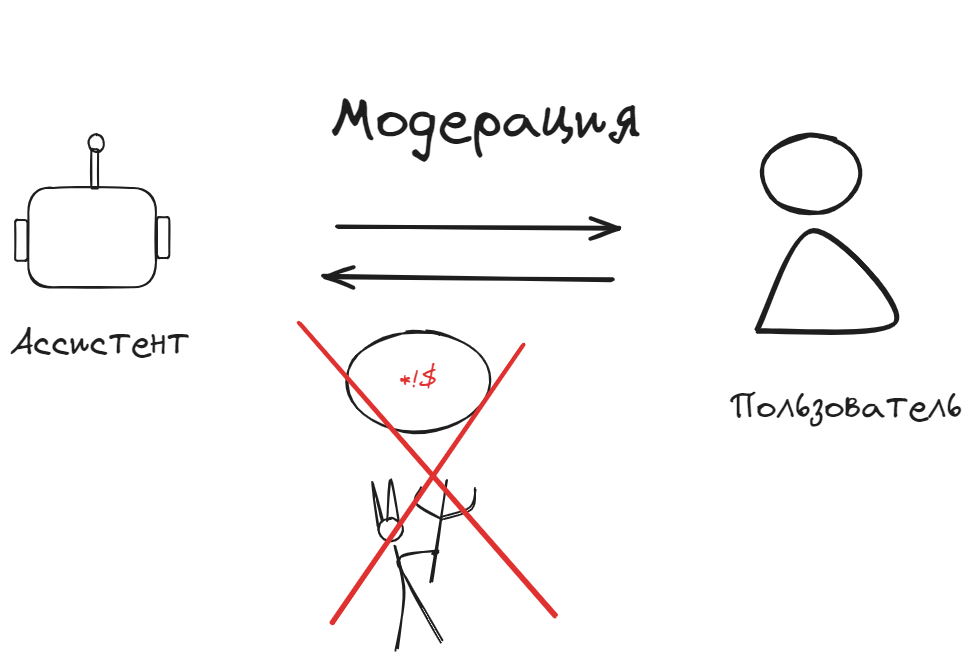
\includegraphics[width=0.5\textwidth]{assets/work/arch/detox.excalidraw.png}
    \caption{Модули PyMorphy \cite{Korobov2015morph} и CLIP позволяют исключить неэтичное общение и изображение }
    \label{detox}
\end{figure}








